\clearpage

%%%%%%%%%%%%%%%%%%%%%%%
\section{Summary}
%%%%%%%%%%%%%%%%%%%%%%%

\begin{figure}[htbp]
    \centering
    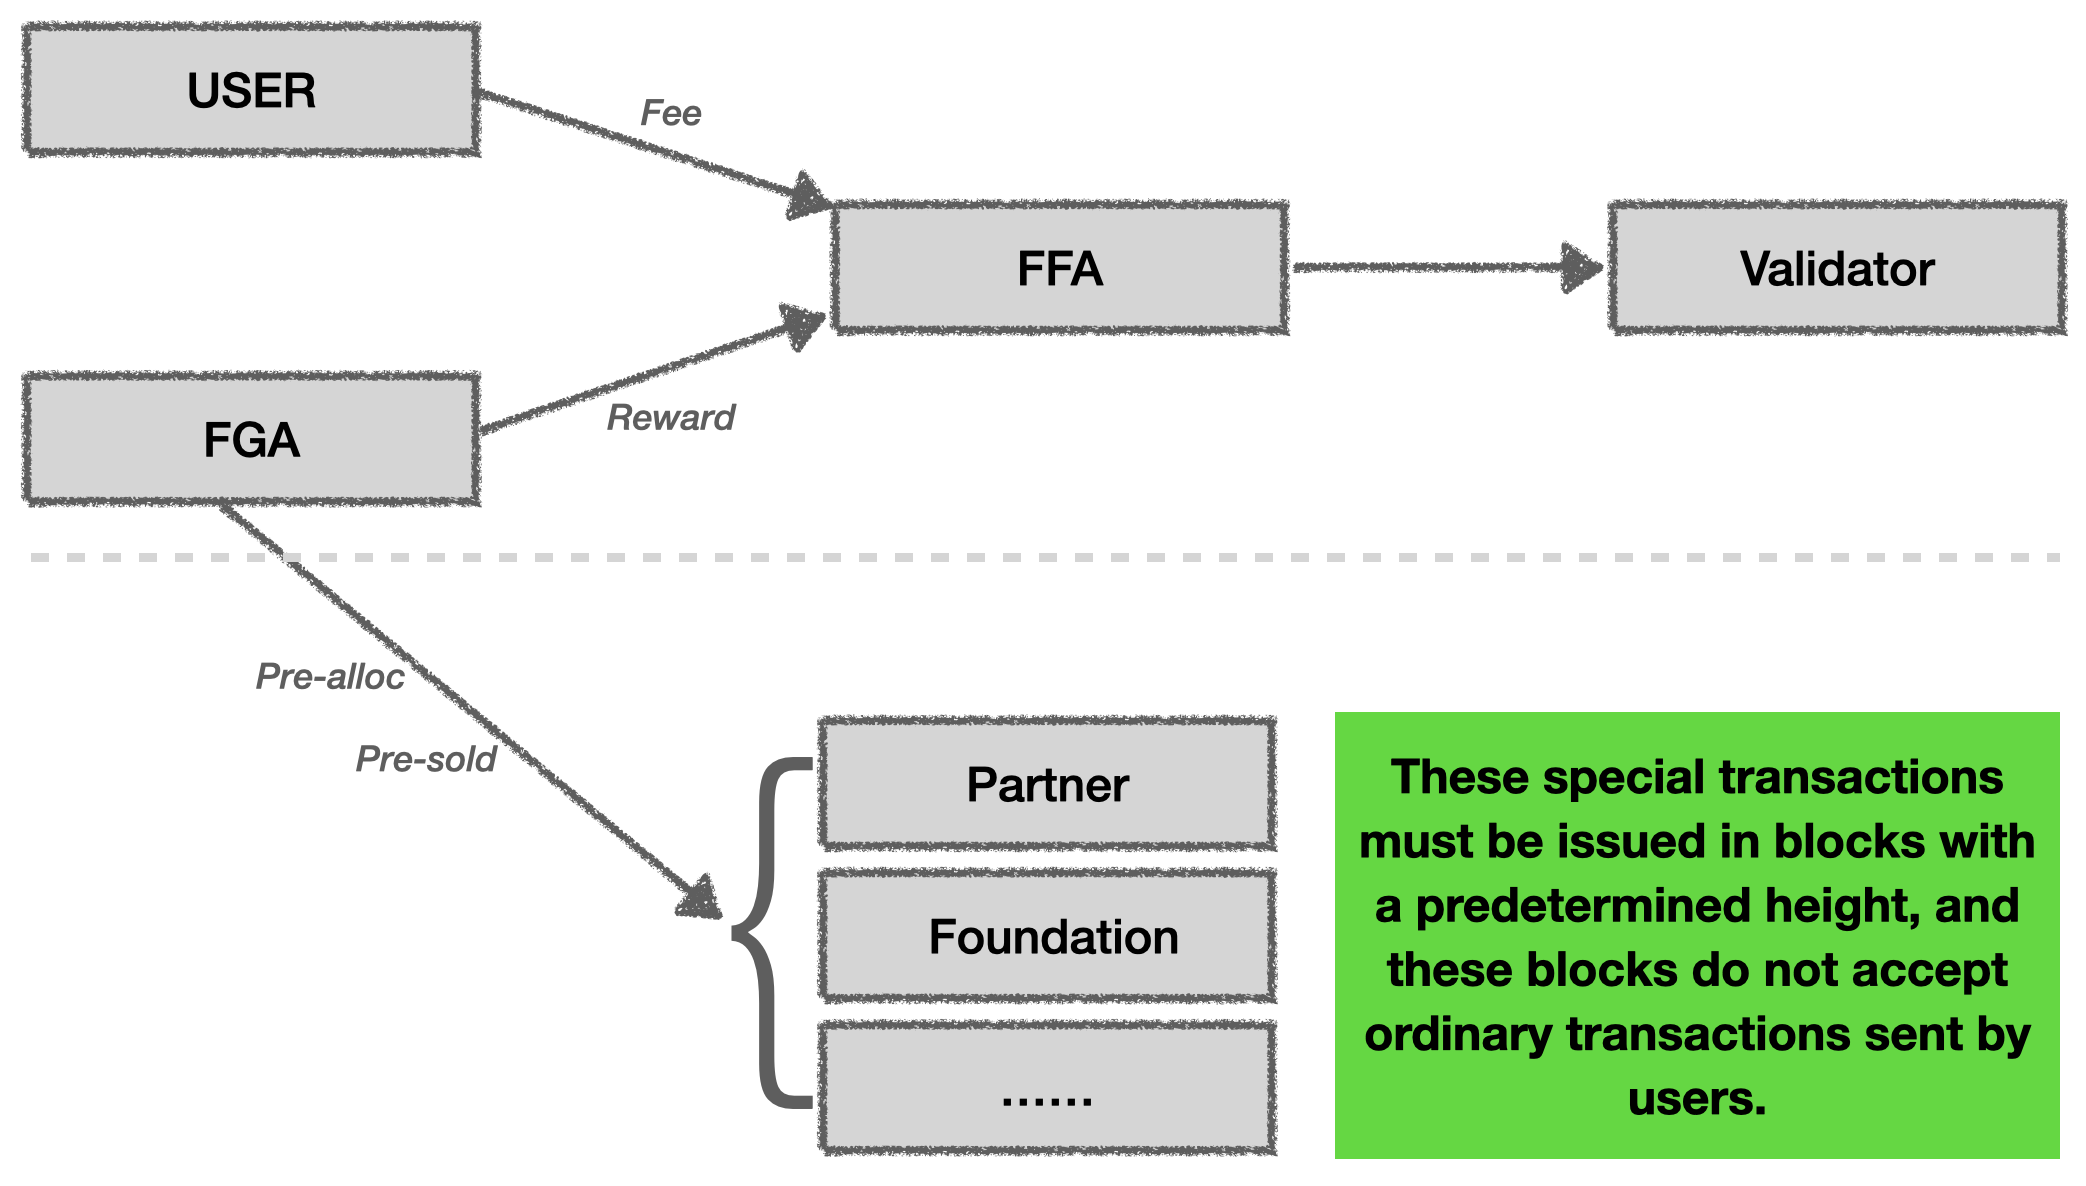
\includegraphics[width=0.9 \textwidth]{/Users/fh/fgr/src/pics/postflow.png}
    \caption{Findora Asset Management}
\end{figure}

~\par

Finally, organize all necessary tasks into a list:

~\par

\begin{ENUMERATE}
\item define a \LSTINLINE{FFA} and a \LSTINLINE{FGA} with their \LSTINLINE{XfrKeyPair} known to all
    \item add some special logics to check transactions related to the \LSTINLINE{FFA}
    \item for each block, at most one transaction can do transfer from the \LSTINLINE{FFA} to outside
    \item create a customed \LSTINLINE{txn_builder} static library for \LSTINLINE{Go FFI}
    \item add necessary codes in the \LSTINLINE{Tendermint} to support the logics mentioned above
\end{ENUMERATE}